\section{\sysname~Design}
\label{sec:slimmer}

%Our analysis in Section~\ref{sec:redundant_files} suggests that adding the
%support of file-level deduplication to Docker registry can significantly reduce
%its storage capacity requirements, especially in large-scale deployments.
%
%In this section, we first describe a high-level design of \emph{\sysname}---
%a Docker registry that supports file-level deduplication.
%We then proceed with a simulation-based evaluation of the expected performance
%implications.
%Integrated Caching and Deduplication
%Cache-assisted Inline deduplication system


%In this section, we first present the challenges brought by the unique characteristics of the Docker ecosystem.
%Next, we discuss our design goals and finally present the design of~\sysname. 
%Then we present the design of~\sysname. 
%O are to improve Docker registry performance and to decrease the backend storage requirements such as ???.

\vspace{-4pt}
\subsection{Registry Deduplication \& Caching}
\label{sec:design}
\vspace{-4pt}

%\sysname\ performs file-level deduplication for a Docker registry.
%

%We designed \sysname\ so that the interface between the Docker clients and the
%registry remains unchanged.
%
%As such, no modifications to the Docker clients are needed.
%
%Below we describe how \sysname\ handles layer pushes and
%pulls at the registry side.
%
%For the sake of this paper, we explain only the main steps omitting smaller
%details.
%\Ali{Following text makes no sense.. what are you trying to explain??}
%\NZ{This part includes our architecture. Our architecture doesn't required many words to explain}
%
%Traditionally, Docker registry is a web server that serves Docker
%\texttt{pull} and Docker \texttt{push} requests.  Although Docker registry is a
%layer-level content addressable storage system holding all the images, it
%delegates storage to drivers which interact with either a local file system or
%a remote cloud storage like S3~\cite{xxx}, Microsoft Azure~\cite{xxxx}, OpenStack Swift~\cite{xxx}, and Aliyun
%OSS~\cite{xxx} as shown in Figure~\ref{fig:sys-overview}.
%Deduplication methods are implemented on remote cloud storage servers or data centers to
%transparently remove duplicates from the incoming data stream.

%proxy caches, or web/HTTP caches 
%Modern container registries such as Google Container Registry~\cite{GoogleContainerRegistry} use cloud storage as their backend Docker image storage systems. 
%Users push and pull Docker images to and from their repositories stored on cloud storage. 
%
%To facilitate a fast and high-availability service, container registries use regional private repositories across the world.  
%This geographical distribution allows users to store images close to their compute instances and experience a fast response time. 
%For example, IBM's Container Registry setup spans five regions~\cite{dockerworkload}. 

%caches are placed as close to the requesting client as possible,
%such caches are known as for the temporary
%storage of frequently requested data to reduce the server's lag.  They are
%typically deployed in a regional ISP or within a corporate network.

\sysname~seamlessly integrates 
%the management of 
caching and deduplication on the
backend storage system (\emph{backend dedup storage}) with Docker registries.
%
We address a set of unique challenges to enable this integration.
%
First, for caching layers, \texttt{pull} layer requests are difficult to
predict because layers are accessed infrequently.
In~\cref{sec:background},
%\arb{???}, 
we have observed that about half of the layers are not
accessed again for at least $1.3$~hours. This means that if we
cache a layer, we may need to wait a long time before we observe a hit on that layer (as discussed in~\cref{sec:background}).  
This is mainly 
because when a user pulls an image from the registry, the Docker daemon on the
requesting host will only pull the layers that are not locally stored.
%\Ali{I do not understand the following sentence.}
%Moreover, we have to consider that a user might deploy an applications on
%multiple machines, so it's not easy to predict when a user will access which layers. 
%%\Ali{The above statement is incorrect. You have to distinguish between GET layer requests
%that are issued after a (PUSH layer + GET manifest) request and a normal GET layer request.
%FAST paper only talk about case 1. Whereas you are generalizing that any GET layer request
%should have a precedent GET layer request which is wrong. We can make a case
%that not all GET layers requests have a precedent PUSH layer request but we can
%not say that it takes a few days, weeks, or even months for a user to make a pull
%layer request after a push layer request.}
%\NZ{I mean the first case, push beyond your trace collection time.}
%

Second, we can not deduplicate compressed layers. For deduplication, each layer
needs to be uncompressed, and only then can undergo file-level deduplication. Similarly,
to restore a layer, we need to fetch files from multiple servers, and only then compress
them in to a tar file to serve a \texttt{pull} layer request. 
%\arb{that can service the ??? request}\NZ{addressed}. 
This whole process can incur a 
considerable performance overhead on \texttt{pull} layer requests.
Deduplication also slows down
\texttt{push} layer requests because of its high demand for CPU, memory, I/O, and network resources.
%\Ali{Explain how push layer requests are not effected?}\NZ{fixed}

%\subsection{Design}
To address these issues, we propose a new registry design. The key feature of our design is a user access history-based prefetching cache that helps mitigate the performance degradation due to the 
backend dedup storage system (Figure~\ref{fig:sys-overview}). Based
on layer access pattern we observed in~\cref{sec:background} and user access history information,
\sysname precisely prefetch the layers that will be pulled shortly.
%has not been pulled in the requested repository
%and the prefetched 
%In this case, we can   
%a user's active time is predictable. 
%Thus, we leverage users' behavior, \ie
%when a user is most likely to be active, to drive layer evictions from the cache.

\begin{figure*}[t]
	\centering
		%\begin{minipage}{0.225\textwidth}
			\centering
			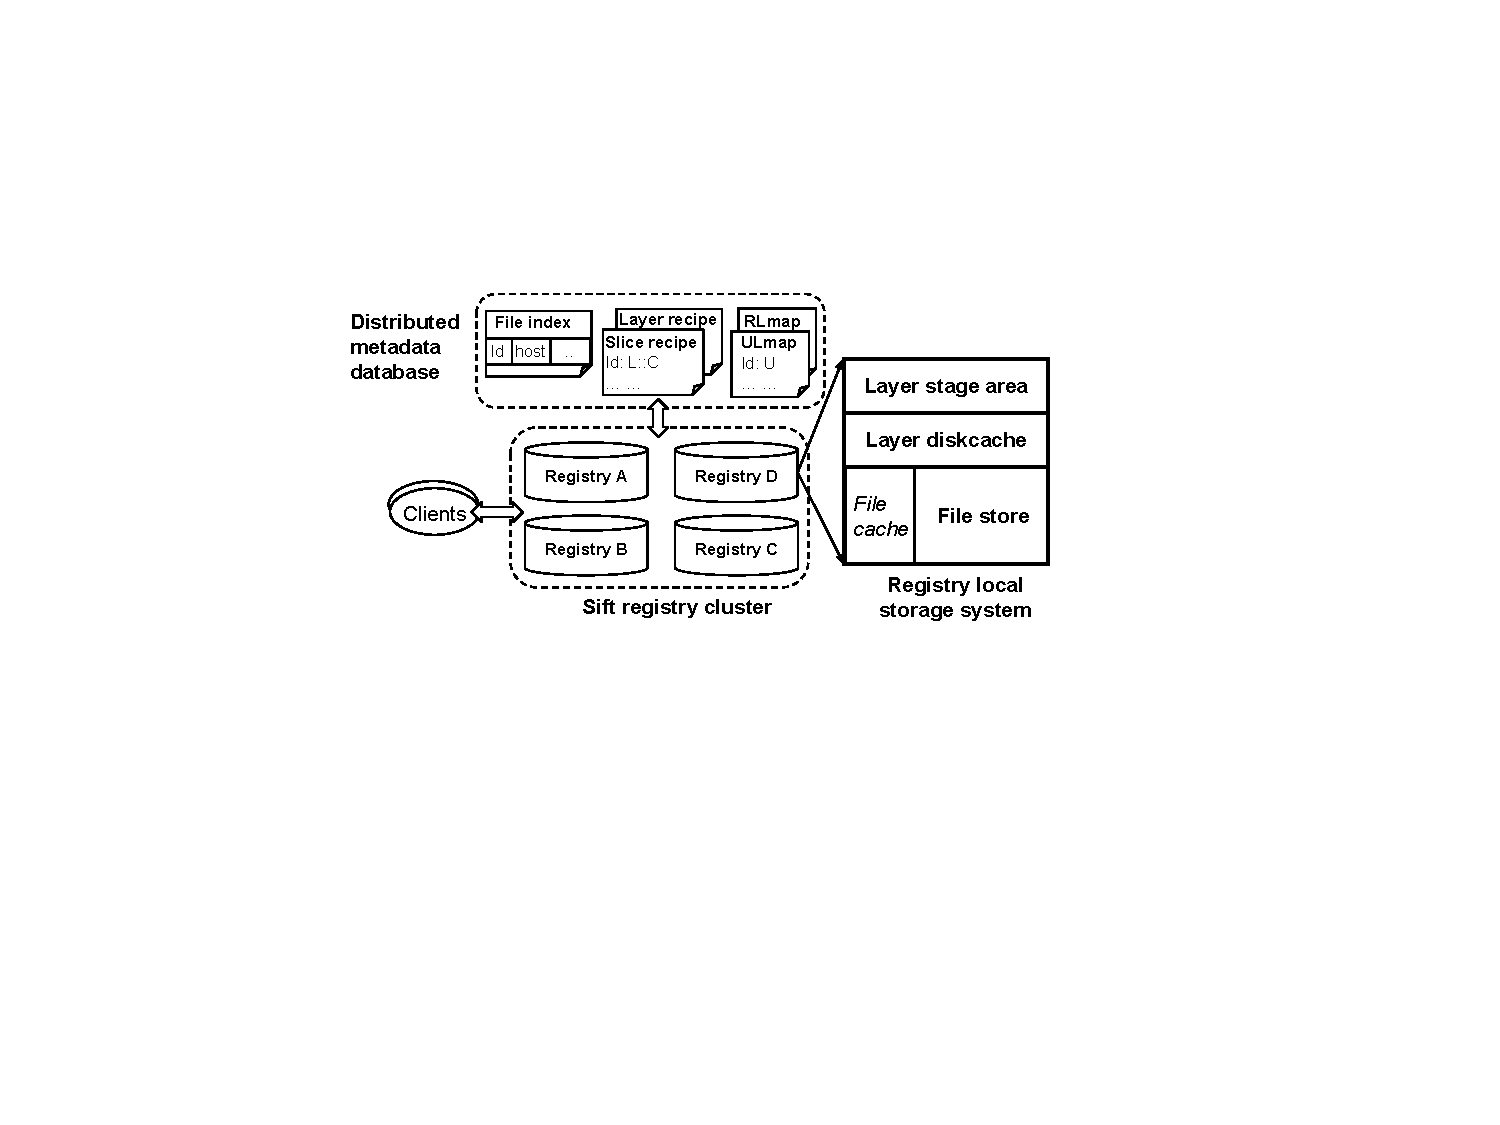
\includegraphics[width=0.9\textwidth]{graphs/sys-architecture.pdf}
%\vspace{-4pt}
			\caption{Architecture of \sysname.}
			%\label{fig:ref_count}
		%\end{minipage}
%	\begin{minipage}{0.225\textwidth}
%		\centering
%		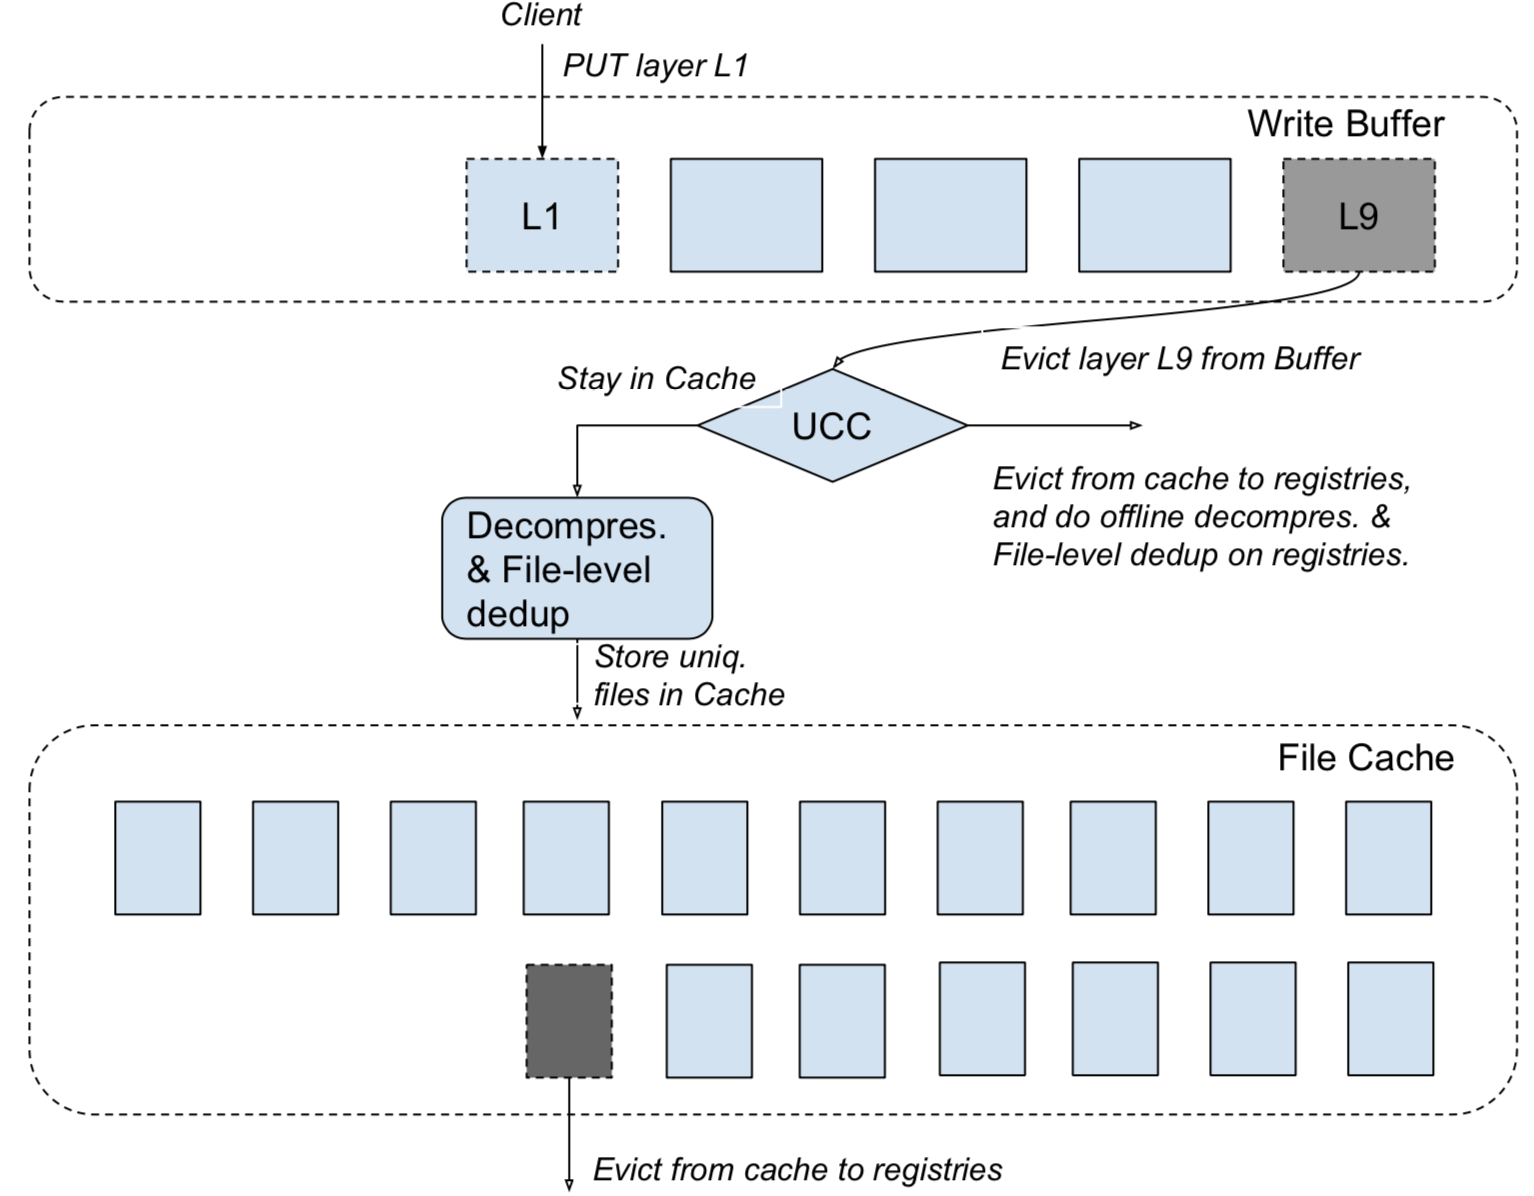
\includegraphics[width=1\textwidth]{graphs/slimmer-cache.png}
%		\caption{CDF of compress. and uncompress. layer size.}
%		\vspace{-3pt}
		\label{fig:sys-overview}
%\vspace{-4pt}
%	\end{minipage}
\end{figure*}


Considering that layer sizes are typically about several MB~\cite{dockerworkload}, 
a small main memory cache will be unable to accommodate
all prefetched layers for all active users. 
To address this issue, we 
create separate caches for layers and \emph{unique} files, called {\em layer buffer} and {\em file cache}, respectively. 
%Both caches comprise both
%main memory and flash memory.
%Layer buffer
%\arb{are main memory for one type and flash for the other type, or both for both types. I assumed both types of memory are used, and there are two caches. check previous sentence for correctness.}\NZ{addressed}
Note that, layers are  compressed tarballs and buffered in layer buffer, and 
%sent by users
 \emph{unique} files are uncompressed files from which duplicates have been removed and stored on flash-based storage. 
%We call compressed layer cache and \emph{deduped} files cache,
%\emph{layer buffer} and \emph{file cache}, respectively.
For 
cache evictions, we first evict inactive users' layers from the layer buffer.
Next, we \emph{dedup} the evicted layers, then store the \emph{unique} files
into the file cache (detailed in~\cref{sec:design_operations}). 
%the following operations: decompressing each evicted layer and comparing its
%containing files with the files that are already stored in the file cache,
%eliminating duplicate files, that is, only storing the unique files on flash
%storage.

When a user requests a
layer that is not present in the layer buffer, the request is forwarded to the
file cache (detailed in~\cref{sec:design_operations}). 
If a layer is also not found in the
file cache, the request is forwarded to the backend dedup storage system.
Note that after layer deduplication, unique files are
scattered across multiple servers. 
We define all the per-server files belonging to a layer as a {\em slice}. 
A server stores slices for many layers, and a layer is composed of slices stored on multiple servers.
To avoid the network latency caused by fetching slices from different servers and
assembling them into a whole compressed layer, we split a \texttt{pull} request 
into several~\texttt{pull slice}~requests. Those requests will then be
forwarded to all the backend servers that store the requested
layer's slices. 
After a~\texttt{pull slice}~request is received, each backend server compresses the slice 
and directly sends it back to the user.
We modify the Docker client
interface such that when it receives all the compressed slices, it can
decompress them into a single layer. 
Furthermore, compressing slices
of layers in parallel considerably mitigates the compression latency caused by
compressing a whole layer, since compression time depends on the size of the
uncompressed data.
%to cache layers and cache unique files after decompression and deduplication,
%respectively.  consists of a \emph{layer buffer} and a \emph{file cache}.  The
%layer buffer stores all the newly pushed layers in memory.  Although accessing
%memory is very fast, the size of main memory is limited. 
%All the slices for a layer are fetched in parallel for performance improvement.



 


\subsection{Operations}
\label{sec:design_operations}

%\paragraph{Workflow}
%
The proposed Docker registry API is very similar to the original registry.
%Interactions with the Docker client is unchanged: 
a user simply pushes and pulls images to and from the registry. 
In the following, we explain Docker operations integration with \sysname.

%\sysname~ is composed of five main components(see Figure~\ref{onshareddir}):
%a modified Docker client,
%layer buffer,
%file cache,
%registries,
%backend storage system that implements deduplication.
%The modified Docker client sends put or pull layer/manifest requests.
%After it sends the pull layer requests.
%it receives multiple partial layers and decompresses them together as a whole uncompressed layer, then verifies the
%integrity of the uncompress layer by calculating the digest of the uncompress layer.
%Layer buffer is used to buffer all the put layer requests and 
%cache prefetched layers for later use.

\textbf{Push.}
After receiving a \texttt{push} layer request from the client, 
\sysname~first buffers the layer in the layer buffer for later accesses. 
The layer buffer can be implemented on a distributed in-memory store,~\eg Plasma~\cite{plasma}.
At the same time, \sysname~will also submit the layer to the backend dedup storage system.
Our layer buffer and file cache use write through policies. 
Since there is no modification to the layer or unique files, 
there is no data consistency issue between the cache and the backend dedup storage system.
A cold layer eviction may be triggered on layers stored in the layer buffer.
The cold layer will be evicted to the file cache, but before that can happen, it will be \emph{deduped}.
The deduplication process includes the following steps 
that are applied on every victim layer evicted from the layer buffer to the file cache:

\begin{compactenumerate}
	\item decompress and unpack the layer's tarball into individual files;
	\item compute a \emph{fingerprint} for every file in the layer;
	\item check every file's fingerprint against the \emph{fingerprint index} to
	identify if identical files are already present in the file cache;
	\item only store the unique files in the file cache and update the 
	\emph{file index} with the unique files' fingerprints, location, and its host address;
	\item create and store a \emph{layer recipe} that includes the file path,
	metadata, and fingerprint of every file in the layer; and
	\item remove the layer's tarball from the layer buffer, completing eviction.
\end{compactenumerate}

Layer recipes are identified by layer digests, and files are identified by their fingerprints.
These identifiers are used to address corresponding objects in the underlying flash storage. 
Fingerprint index and layer recipes are stored on Redis~\cite{redis}.

File cache is a flash-based distributed cache that can be implemented on 
distributed log structured store, \eg CORFU~\cite{180277}.
The unique files are flash-friendly because there is no modification to these files.
%, meaning that there is no small write.?
%
%Usually, the underlying distributed flash-based stores such as CORFU transparently spread data among 
%different servers and upper level applications are unaware of data host address. 
%We modified CORFU's read and write interfaces so that the file locations and 
%its host addresses are exposed to our ~\sysname.
%
%Similar to layer buffer, storing unique files in file cache might also trigger the eviction of cold layer's files.
The eviction of a cold layer from the layer buffer to file cache
 may also trigger the eviction of unique files in file cache.
Since the backend dedup storage system already stores a backup of the layers, 
we can simply discard the victim files from the file cache. Algorithm~\ref{alg:cache} presents our 
cache replacement algorithm.
%\sysname\ handles push requests asynchronously.
%\sysname 
%does not immediately unpack the layer.
%Instead, it reliably stores the layer's compressed tarball in a persistent
%\emph{staging area}.
%A separate \emph{off-line} deduplication process iterates over the layers in
%the staging area and performs the following steps for every layer:
%%
%\begin{compactenumerate}
%	\item decompress and unpack the layer's tarball into individual files;
%	\item compute a \emph{fingerprint} for every file in the layer;
%	\item check all file fingerprints against the \emph{file index} to
%	identify if identical files are already stored in \sysname;
%	\item store non-deduplicated files in \sysname's storage;
%	\item create and store a \emph{layer recipe} that includes the path,
%	metadata, and fingerprint of every file in the layer;
%	\item remove the layer's tarball from the staging area.
%\end{compactenumerate}

%The advantage of off-line deduplication is that it keeps push
%latencies perceived by the Docker clients low.
%
%The background deduplication process can be scheduled during the periods of low
%load on the registry.
%
%Layer recipes are identified by layer digests (see Section~\ref{sec:background})
%and files are identified by their fingerprints.
%%
%These identifiers are used to address corresponding objects in the
%underlying storage.
%
%For example, if a file system is used as a backend storage, \sysname\ creates a
%single file for every layer recipe (named by the digest) and a single file for
%every in-layer file (named by the fingerprint).

\paragraph{Pull}
A \texttt{pull} layer request that can be serviced from the 
layer buffer is a layer buffer hit and does not need further action. 
In case of a miss in the layer buffer, the needed files may be found in the 
file cache. In this happens, 
 \sysname~\emph{reconstructs} the layer from the file cache according to the layer recipe.
%
%A pull request cannot be postponed to an off-line process as the
%pulling client is actively waiting for the layer.
%
The layer reconstruction from the file cache involves the following steps that are performed \emph{inline}:

\begin{compactenumerate}
	%\item check if the requested layer is still in the staging area and if so,
	%service it directly from there;
	\item find the layer recipe using the layer digest and retrieve the 
\emph{fingerprints} for the files associated with the layer;
	\item lookup the \emph{fingerprints} in \emph{fingerprint index} to get a destination server list; and
	\item forward the \texttt{pull slice} layer request and layer recipe to each server in the server list.
\end{compactenumerate}

Once the \texttt{pull slice} layer request is received, each destination server will initiate a layer slice restoring process. This process involves  
the following steps: 

\begin{compactenumerate}
	\item prepare a directory structure for the layer, based on the layer recipe;
	\item copy the locally available files into the directory tree; 
	\item compresses the layer's directory tree into a temporary tarball; and
	\item send the layer tarball back to the client, and then discard the tarball.
\end{compactenumerate}

If a \texttt{pull} layer request results in a miss in both the layer buffer and the file cache, 
the request will be forwarded to the backend dedup storage system.
The layer restoring process on the backend storage system is similar to restoring from the file cache.
Many modern storage systems with the deduplication feature can be used as our backend storage system, including GFS~\cite{ghemawat2003google}, HDFS~\cite{hdfs}, S3~\cite{s3}, and Swift~\cite{swift}.
We can modify the above systems so that they can recognize the compressed layer file type and decompress them before performing deduplication.
Moreover, these systems need to be modified to restore layer slices in parallel. 
%Note that there is no consistency issue between either layer buffer, file cache or backend storage because layers won't be changed in the future.





